\subsection{\texorpdfstring{同态 \(\mathbf{E}^* \otimes_{\mathbf{A}} \mathbf{F} \to \operatorname{Hom}_{\mathbf{A}}(\mathbf{E}, \mathbf{F})\)}{同态 \textbackslash mathbf\{E\}\^{}* \textbackslash otimes\_\{\textbackslash mathbf\{A\}\} \textbackslash mathbf\{F\} \textbackslash 到 \textbackslash operatorname\{Hom\}\_\{\textbackslash mathbf\{A\}\}(\textbackslash mathbf\{E\}, \textbackslash mathbf\{F\})}}

设 A、B 为两个环，E 为左A-模，F 为左B-模，G 为 (A, B)-双模。Z-模 \(\operatorname{Hom}_{\mathbf{A}}(\mathbf{E}, \mathbf{G})\) 典范地具有一个右B-模结构（§1，第14号），使得 \((u\beta)(x) = u(x)\beta\)（对 \(\beta \in \mathbf{B}\)、\(u \in \operatorname{Hom}_{\mathbf{A}}(\mathbf{E}, \mathbf{G})\)、\(x \in \mathbf{E}\)）。另一方面，\(\mathbf{G} \otimes_{\mathbf{B}} \mathbf{F}\) 典范地具有一个左A-模结构（§3，第4号）。我们将定义一个典范 \(\mathbf{Z}\)-同态

\[
\nu : \operatorname{Hom} _ {\mathbf {A}} (\mathrm{E}, \mathrm{G}) \otimes_ {\mathbf {B}} \mathrm{F} \rightarrow \operatorname{Hom} _ {\mathbf {A}} (\mathrm{E}, \mathrm{G} \otimes_ {\mathbf {B}} \mathrm{F}).\tag{7}
\]

为此，对于所有 \(y \in \mathbf{F}\) 以及所有 \(u \in \operatorname{Hom}_{\mathbf{A}}(\mathbf{E}, \mathbf{G})\)，我们考虑映射 \(\nu'(u, y): x \mapsto u(x) \otimes y\)（从 \(\mathbf{E}\) 到 \(\mathbf{G} \otimes_{\mathbf{B}} \mathbf{F}\)）。立即可以验证，\(\nu'(u, y)\) 是 A-线性的，且 \(\nu'\) 是从 \(\operatorname{Hom}_{\mathbf{A}}(\mathbf{E}, \mathbf{G}) \times \mathbf{F}\) 到 \(\operatorname{Hom}_{\mathbf{A}}(\mathbf{E}, \mathbf{G} \otimes_{\mathbf{B}} \mathbf{F})\) 的 Z-双线性映射；此外，对所有 \(\beta \in \mathbf{B}\)，\(\nu'(u\beta, y)\) 与 \(\nu'(u, \beta y)\) 相等，因为 \((u(x)\beta) \otimes y = u(x) \otimes (\beta y)\)。于是我们得出结论（§3，第1号，命题1）：存在所求的同态 \(\nu\)，使得 \(\nu(u \otimes y)\) 是 A-线性映射 \(x \mapsto u(x) \otimes y\)。

立即可以验证，若E是一个 \((\mathbf{A}, (\mathbf{C}_{i}^{\prime}) ; (\mathbf{D}_{j}^{\prime}))\) -多模，F是一个 \((\mathbf{B}, (\mathbf{C}_{h}^{\prime\prime}) ; (\mathbf{D}_{k}^{\prime\prime}))\) -多模，且G是一个 \((\mathbf{A}, (\mathbf{C}_{l}^{\prime\prime}) ; \mathbf{B}, (\mathbf{D}_{m}^{\prime\prime}))\) -多模，则映射(7)是一个 \(((\mathbf{D}_{j}^{\prime}), (\mathbf{C}_{h}^{\prime\prime}), (\mathbf{C}_{l}^{\prime\prime}) ; (\mathbf{C}_{i}^{\prime}), (\mathbf{D}_{k}^{\prime\prime}), (\mathbf{D}_{m}^{\prime\prime}))\) -多模同态。

命题2. (i) 当F是投射（相应地，有限生成投射）B-模时，典范同态(7)是单射（相应地，双射）。

\begin{enumerate}
\def\labelenumi{(\roman{enumi})}
\setcounter{enumi}{1}
\item
  当E是有限生成的投射A-模时，典范同态(7)是双射的。
\item
  固定E与G，对每个左B-模F，我们记
\end{enumerate}

\[
\mathrm{T} (\mathrm{F}) = \operatorname{Hom} _ {\mathrm{A}} (\mathrm{E}, \mathrm{G}) \otimes_ {\mathrm{B}} \mathrm{F}, \quad \mathrm{T} ^ {\prime} (\mathrm{F}) = \operatorname{Hom} _ {\mathrm{A}} (\mathrm{E}, \mathrm{G} \otimes_ {\mathrm{B}} \mathrm{F});
\]

对每个左B-模同态 \(u: \mathbf{F} \to \mathbf{F}'\)，我们记 \(\mathrm{T}(u) = 1 \otimes u\)（这里的1表示 \(\operatorname{Hom}_{\mathbf{A}}(\mathbf{E}, \mathbf{G})\) 的恒等映射），

\[
\mathrm{T} ^ {\prime} (u) = \operatorname{Hom} \left(\mathrm{l} _ {\mathbb {E}}, \mathrm{l} _ {\mathbb {G}} \otimes u\right);
\]

另一方面，我们用 \(\nu_{F}\) 代替 \(\nu\)。于是我们有以下引理：

引理1. 对于每个同态 \(u: \mathbf{F} \to \mathbf{F}'\) ，该图表

\[
\begin{array}{c c c} \mathrm{T(F)} & \xrightarrow {\nu_ {\mathrm{F}}} & \mathrm {T^ {\prime} (F)} \\ \mathrm{T(u)} \Big \downarrow & & \Big \downarrow \mathrm {T^ {\prime} (u)} \\ \mathrm {T(F^ {\prime})} & \xrightarrow {\nu_ {\mathrm {F^ {\prime}}}} & \mathrm {T^ {\prime} (F^ {\prime})} \end{array}\tag{8}
\]

是交换的。

验证是直接的。

引理2. 设 M, N 是 F 中的两个互补子模，i: M → F, j: N → F 为典范嵌入。图表

\begin{enumerate}
\def\labelenumi{(\arabic{enumi})}
\setcounter{enumi}{8}
\tightlist
\item
\end{enumerate}

\pandocbounded{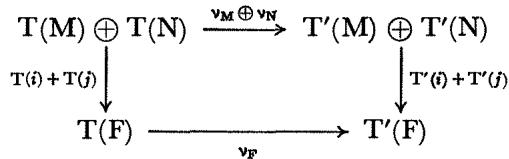
\includegraphics[keepaspectratio]{images/part002_2544dc0c.jpg}}

是可交换的，且竖直箭头是双射。

交换性由引理1得出，其余断言由§1第6号命题6的推论2以及§3第7号命题7得出。

引理3. 在引理2的假设下，\(\nu_{\mathrm{F}}\) 为单射（相应地，满射）的必要且充分条件是 \(\nu_{\mathrm{M}}\) 与 \(\nu_{\mathrm{N}}\) 皆然。

这由引理2及§1第6号命题6的推论1得出。

于是引理3连同§2第2号命题4表明，只需考虑F为自由模的情形。但若 \((b_{\mu})\) 是F的一组基，则 \(\operatorname{Hom}_{\mathbf{A}}(\mathbf{E}, \mathbf{G}) \otimes_{\mathbf{B}} \mathbf{F}\) 的每个元素都可唯一地写成 \(\sum_{\mu} u_{\mu} \otimes b_{\mu}\)，其中 \(u_{\mu} \in \operatorname{Hom}_{\mathbf{A}}(\mathbf{E}, \mathbf{G})\)（§3，第7号，命题7的推论1）；该元素在 \(\nu\) 下的像是 A-线性映射 \(x \mapsto \sum_{\mu} u_{\mu}(x) \otimes b_{\mu}\)；它不可能对所有 \(x \in \mathbf{E}\) 均为零，除非 \(u_{\mu}(x) = 0\)（对所有 \(x \in \mathbf{E}\) 与所有 \(\mu\) 成立），而这等价于 \(u_{\mu} = 0\)（对所有 \(\mu\)）；因此 \(\nu\) 是单射。当F还具有有限基时，引理3表明（通过对F的基中元素个数作归纳），要证明 \(\nu\) 是满射，只需就 \(F = B_s\) 的情形证明即可；但在此情形，(7) 式的两边都典范地等同于 \(\operatorname{Hom}_{\mathbf{A}}(\mathbf{E}, \mathbf{G})\)（§3，第4号，命题4），而 \(\nu\) 成为恒等映射。

\begin{enumerate}
\def\labelenumi{(\roman{enumi})}
\setcounter{enumi}{1}
\tightlist
\item
  为证明E为投射且有限生成时的命题，这次我们固定F与G，并对每个左A-模E记：
\end{enumerate}

\[
\mathrm{T} (\mathrm{E}) = \operatorname{Hom} _ {\mathrm{A}} (\mathrm{E}, \mathrm{G}) \otimes_ {\mathrm{B}} \mathrm{F}, \quad \mathrm{T} ^ {\prime} (\mathrm{E}) = \operatorname{Hom} _ {\mathrm{A}} (\mathrm{E}, \mathrm{G} \otimes_ {\mathrm{B}} \mathrm{F})
\]

并且，对于每一个左A模同态 \(v:\mathbf{E}\to\mathbf{E}^{\prime}\) ,

\[
\mathrm{T} (v) = \operatorname{Hom} (v, 1 _ {\mathbf {G}}) \otimes 1 _ {\mathbf {F}}, \quad \mathrm{T} ^ {\prime} (v) = \operatorname{Hom} (v, 1 _ {\mathbf {G}} \otimes 1 _ {\mathbf {F}});
\]

另一方面，我们用 \(\nu_{E}\) 代替 \(\nu\)。于是我们有以下两个引理：

引理4. 对于每个同态 \(v: \mathbf{E} \to \mathbf{E}'\) ，该图表

\[
\begin{array}{c c c} \mathrm{T} (\mathrm{E} ^ {\prime}) & \xrightarrow {\nu_ {\mathrm{E} ^ {\prime}}} & \mathrm{T} ^ {\prime} (\mathrm{E} ^ {\prime}) \\ \mathrm{T} (v) \Big \downarrow & & \Big \downarrow \mathrm{T} ^ {\prime} (v) \\ \mathrm{T} (\mathrm{E}) & \xrightarrow {\nu_ {\mathrm{E}}} & \mathrm{T} ^ {\prime} (\mathrm{E}) \end{array}\tag{10}
\]

是交换的。

引理5. 设 \(\mathbf{M}\) 与 \(\mathbf{N}\) 是 \(\mathbf{E}\) 中两个互补的子模，\(p: \mathbf{E} \to \mathbf{M}\)、\(q: \mathbf{E} \to \mathbf{N}\) 为典范投影。图表

\pandocbounded{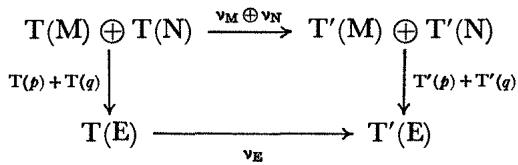
\includegraphics[keepaspectratio]{images/part002_a961576f.jpg}}

是可交换的，且竖直箭头是双射。

它们的证明与引理1和引理2相同，并用到§1第6号命题6的推论2、§2第1号命题1以及§3第7号命题7。

证明的余下部分随后按 (i) 的方式进行，并归结为 \(E = A_{s}\) 的情形；此时 (7) 式的两边典范地等同于 \(G \otimes_{B} F\)，而 \(\nu\) 成为恒等映射。

特别地，取 B = A 且 G 为 (A, A)-双模 \(_{s}A_{d}\)（§3，第4号），于是右A-模 \(\operatorname{Hom}_{\mathbf{A}}(\mathbf{E}, _{s}\mathbf{A}_{d})\) 就是E的对偶E*，并且 \((_{s}\mathbf{A}_{d}) \otimes_{\mathbf{A}} F\) 典范地等同于F（§3，第4号，命题4）。此时同态 (7) 成为典范Z-同态

\[
\theta : \mathrm{E} ^ {*} \otimes_ {\mathrm{A}} \mathrm{F} \rightarrow \operatorname{Hom} _ {\mathrm{A}} (\mathrm{E}, \mathrm{F})\tag{11}
\]

和 \(\theta (x^{*}\otimes y)\) 是E到F的线性映射

\[
x \mapsto \langle x, x ^ {*} \rangle y.
\]

注记（1）. §2 第6号命题12中给出的投射A模的刻画也可表述如下：对于左A模E为投射模，其充分必要条件为典范同态

\[
\theta_ {\mathbf {E}}: \mathrm{E} ^ {*} \otimes_ {\mathbf {A}} \mathrm{E} \rightarrow \operatorname{Hom} _ {\mathbf {A}} (\mathrm{E}, \mathrm{E}) = \operatorname{End} _ {\mathbf {A}} (\mathrm{E})
\]

使得 \(l_{E}\) 属于 \(\theta_{E}\) 的像。

推论. (i) 当F是投射（相应地，有限生成投射）模时，典范同态 (11) 是单射（相应地，双射）。

\begin{enumerate}
\def\labelenumi{(\roman{enumi})}
\setcounter{enumi}{1}
\tightlist
\item
  当E是有限生成投射模时，典范同态(11)是双射的。
\end{enumerate}

即使E与F都是有限生成的，\(\theta\) 也不一定满射，例 A = Z、E = F = Z/2Z 即说明这一点；(11) 式右端非零，但 \(E^{*} = 0\)。另一方面，可以给出E为自由模而 (11) 既非单射又非满射的例子（习题3(b)）。

当E具有有限基 \((e_i)\) 时，\(\theta^{-1}\)（\(\theta\) 的逆同构）可以如下显式求出。设 \((e_i^*)\) 为 \((e_i)\) 的对偶基（§2，第6号）；对所有 \(u \in \operatorname{Hom}(\mathbf{E}, \mathbf{F})\) 以及所有 \(x = \sum_{i} \xi_i e_i\)（其中 \(\xi_i \in \mathbf{A}\)），

\[
u (x) = \sum_ {i} \xi_ {i} u (e _ {i}) = \sum_ {i} \langle x, e _ {i} ^ {*} \rangle u (e _ {i})
\]

，从而 \(u = \sum_{i} \theta(e_i^* \otimes u(e_i))\)，换言之

\[
\theta^ {- 1} (u) = \sum_ {i} e _ {i} ^ {*} \otimes u (e _ {i}).\tag{12}
\]

特别地，若进一步有 F = E，则可看出 \(\theta_{E}^{-1}\) 把恒等映射 \(l_{E}\) 映为元素 \(\sum_{i} e_{i}^{*} \otimes e_{i}\)，因此该元素与E中所考虑的基 \((e_{i})\) 无关。

另一方面，注意当E是有限生成投射模时，\(\operatorname{End}_{\mathbf{A}}(\mathbf{E})\) 上的环结构可以通过 \(\theta_{E}^{-1}\) 转移到 \(E^{*}\otimes_{A}E\) 上；立即可以验证，对E中的 x, y 与 \(x^{*}, y^{*}\)（\(E^{*}\) 中的元素），在环 \(\operatorname{End}_{\mathbf{A}}(\mathbf{E})\) 中

\[
\theta_ {\mathbf {E}} (x ^ {*} \otimes x) \circ \theta_ {\mathbf {E}} (y ^ {*} \otimes y) = \theta_ {\mathbf {E}} ((y ^ {*} \langle y, x ^ {*} \rangle) \otimes x).\tag{13}
\]

注记 (2). 设 E 为右 A-模；在 (11) 中用 E* 替换 E，我们得到一个典范的 Z-同态

\[
\mathrm{E} ^ {* *} \otimes_ {\mathrm{A}} \mathrm{F} \rightarrow \operatorname{Hom} _ {\mathrm{A}} (\mathrm{E} ^ {*}, \mathrm{F}).\tag{14}
\]

另一方面，存在一个典范的 A-同态 \(c_{E}:E\to E^{**}\) ，由此得到一个 Z-同态 \(c_{E}\otimes l_{F}:E\otimes_{A}F\to E^{**}\otimes_{A}F\) ；将后者与同态 (14) 复合，我们从而得到一个典范的 Z-同态

\[
\theta^ {\prime}: \mathrm{E} \otimes_ {\mathrm{A}} \mathrm{F} \rightarrow \operatorname{Hom} _ {\mathrm{A}} (\mathrm{E} ^ {*}, \mathrm{F})\tag{15}
\]

使得 \(\theta'(x \otimes y)\) 是线性映射

\[
x ^ {*} \mapsto \langle x, x ^ {*} \rangle y.
\]

若 E 与 F 为投射模，则映射 (15) 是单射。因为 \(c_{E}\) 此时是单射（§2，第 7 号，命题 13 的推论 4），且由于 F 是投射的，Z-同态 \(c_{E} \otimes l_{F}: E \otimes_{A} F \to E^{**} \otimes_{A} F\) 也是单射（§3，第 7 号，命题 7 的推论 6）；最后，已见（命题 2）同态 (14) 是单射，由此得结论。

若 E 是投射且有限生成的，则映射 (15) 是双射，因为构成它的两个映射此时均为双射（§2，第 7 号，命题 13 的推论 4 及上文命题 2）。

